% Needs 2 passes, as the overlay is used!
\documentclass[margin=2pt]{standalone}
\usepackage[table]{xcolor}
\usepackage[utf8]{inputenc}
\usepackage[T1]{fontenc}

\usepackage{tikz}
\usepackage{helvet}
\usepackage{amsmath}

\renewcommand\familydefault\sfdefault

% Use \phantom to hide text for exams
\renewcommand{\phantom}{}
\newcommand{\lOS}{\phantom{Operační}\\\phantom{systém}}
\newcommand{\lTask}{{úloha}}
\newcommand{\lPage}{{stránka}}
\newcommand{\lFreeSpace}{{volný blok}}

\usetikzlibrary{intersections, shapes.arrows, spath3, shapes.geometric, fit, backgrounds, calc, tikzmark}

\definecolor{themeBlue}{RGB}{1, 103, 143}
\definecolor{themeOrange}{RGB}{221, 109, 16}
\definecolor{themeTeal}{RGB}{18, 54, 69}
\definecolor{themeGrey}{RGB}{120, 121, 124}

\begin{document}
    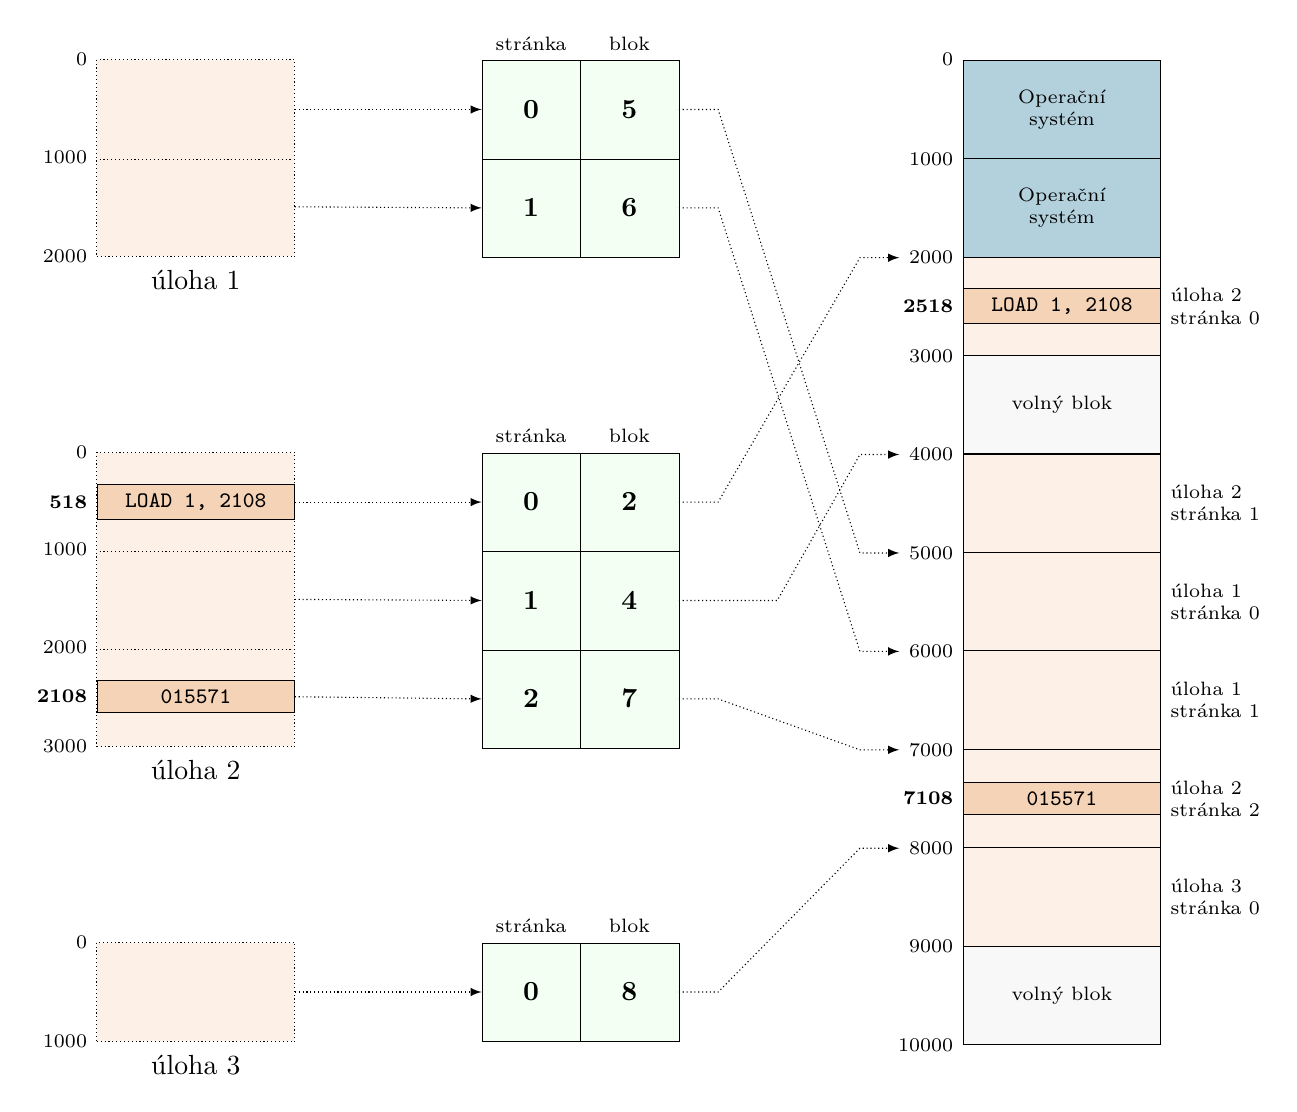
\begin{tikzpicture} [
        width/.style={minimum width=2.5cm},
        mem/.style={draw, width, anchor=north, align=center, minimum height=1.25cm, font=\scriptsize, yshift=\pgflinewidth},
        label left/.style={font=\scriptsize, align=right, left},
        label right/.style={font=\scriptsize, right, align=left},
        label above/.style={font=\scriptsize, above, align=center},
        brace mirror/.style={decoration={brace,mirror,raise=5pt}, decorate},
        brace/.style={decoration={brace,raise=5pt}, decorate},
        os/.style={fill=themeBlue!30},
        free/.style={fill=themeGrey!5},
        task/.style={fill=themeOrange!10},
        block/.style={draw, minimum size=1.25cm, fill=green!5, ultra thin, font=\bfseries},
        cell os/.style={os, node contents={\lOS}},
        cell free/.style={free, node contents={\lFreeSpace}},
        cell task/.style={task, node contents={}},
    ]

    % TASK 1
    \draw node[mem, task, draw=none] (task 1 seg 0) {};
    \draw(task 1 seg 0.south) node[mem, task, draw=none, yshift=\pgflinewidth] (task 1 seg 1) {};
    \node[fit=(task 1 seg 0) (task 1 seg 1), draw, densely dotted, inner sep=0pt] (task 1) {};

    \draw (task 1 seg 1.south) ++(0, -.3) node {\lTask\space1};
    \draw[densely dotted] ($ (task 1 seg 0.south west) + (1pt, 0) $) -- ($ (task 1 seg 0.south east) - (1pt, 0) $);
    \draw (task 1 seg 0.north west) node[label left] {0};
    \draw (task 1 seg 1.north west) node[label left] {1000};
    \draw (task 1 seg 1.south west) node[label left] {2000};

    % TASK 2
    \draw (task 1 seg 1.south) ++(0, -2.5cm) node[mem, task, draw=none] (task 2 seg 0) {};
    \draw(task 2 seg 0.south) node[mem, task, draw=none, yshift=\pgflinewidth] (task 2 seg 1) {};
    \draw(task 2 seg 1.south) node[mem, task, draw=none, yshift=\pgflinewidth] (task 2 seg 2) {};
    \node[fit=(task 2 seg 0) (task 2 seg 1) (task 2 seg 2), draw, densely dotted, inner sep=0pt] (task 2) {};

    \draw (task 2 seg 2.south) ++(0, -.3) node {\lTask\space2};
    \draw[densely dotted] ($ (task 2 seg 0.south west) + (1pt, 0) $) -- ($ (task 2 seg 0.south east) - (1pt, 0) $);
    \draw[densely dotted] ($ (task 2 seg 1.south west) + (1pt, 0) $) -- ($ (task 2 seg 1.south east) - (1pt, 0) $);
    \draw (task 2 seg 0.north west) node[label left] {0};
    \draw (task 2 seg 1.north west) node[label left] {1000};
    \draw (task 2 seg 2.north west) node[label left] {2000};
    \draw (task 2 seg 2.south west) node[label left] {3000};

    % TASK 3
    \draw (task 2 seg 2.south) ++(0, -2.5cm) node[mem, task, draw=none] (task 3 seg 0) {};
    \node[fit=(task 3 seg 0), draw, densely dotted, inner sep=0pt] (task 3) {};

    \draw (task 3 seg 0.south) ++(0, -.3) node {\lTask\space3};
    \draw (task 3 seg 0.north west) node[label left] {0};
    \draw (task 3 seg 0.south west) node[label left] {1000};

    % page - block matrix
    \draw (task 1 seg 0.east) ++(3, 0) node[block] (task 1 page 0 0) {0};
    \draw (task 1 page 0 0.east) node[block, anchor=west, xshift=-\pgflinewidth] (task 1 page 0 1)  {5};
    \draw (task 1 page 0 0.south) node[block, anchor=north, yshift=\pgflinewidth] (task 1 page 1 0) {1};
    \draw (task 1 page 1 0.east) node[block, anchor=west, xshift=-\pgflinewidth] (task 1 page 1 1)  {6};

    \draw (task 2 seg 0.east) ++(3, 0) node[block] (task 2 page 0 0) {0};
    \draw (task 2 page 0 0.east) node[block, anchor=west, xshift=-\pgflinewidth] (task 2 page 0 1)  {2};
    \draw (task 2 page 0 0.south) node[block, anchor=north, yshift=\pgflinewidth] (task 2 page 1 0) {1};
    \draw (task 2 page 1 0.east) node[block, anchor=west, xshift=-\pgflinewidth] (task 2 page 1 1)  {4};
    \draw (task 2 page 1 0.south) node[block, anchor=north, yshift=\pgflinewidth] (task 2 page 2 0) {2};
    \draw (task 2 page 2 0.east) node[block, anchor=west, xshift=-\pgflinewidth] (task 2 page 2 1)  {7};

    \draw (task 3 seg 0.east) ++(3, 0) node[block] (task 3 page 0 0) {0};
    \draw (task 3 page 0 0.east) node[block, anchor=west, xshift=-\pgflinewidth] (task 3 page 0 1)  {8};

    % task -> pb matrix
    \draw[-latex, densely dotted] (task 1 seg 0.east) -- (task 1 page 0 0.west);
    \draw[-latex, densely dotted] (task 1 seg 1.east) -- (task 1 page 1 0.west);
    \draw (task 1 page 0 0.north) node[label above] {stránka};
    \draw (task 1 page 0 1.north) node[label above] {blok};

    \draw[-latex, densely dotted] (task 2 seg 0.east) -- (task 2 page 0 0.west);
    \draw[-latex, densely dotted] (task 2 seg 1.east) -- (task 2 page 1 0.west);
    \draw[-latex, densely dotted] (task 2 seg 2.east) -- (task 2 page 2 0.west);
    \draw (task 2 page 0 0.north) node[label above] {stránka};
    \draw (task 2 page 0 1.north) node[label above] {blok};

    \draw[-latex, densely dotted] (task 3 seg 0.east) -- (task 3 page 0 0.west);
    \draw (task 3 page 0 0.north) node[label above] {stránka};
    \draw (task 3 page 0 1.north) node[label above] {blok};

    % Memory block
    \begin{scope}[xshift=11cm]
        \coordinate (h 0) at (0, 0);
        \foreach \style [count=\n from 1, remember=\n as \lastn (initially 0)] in {os,os,task,free,task,task,task,task,task,free} {
            \draw (h \lastn) node[mem, cell \style, name=mem \n];
            \pgfmathtruncatemacro{\addr}{\n * 1000}
            \draw (mem \n.south west) node[label left] (mem \n\space label) {\addr};
            \coordinate (h \n) at (mem \n.south);
        }
        \draw (mem 1.north west) node[label left] (mem 0 label) {0};
    \end{scope}

    % block -> memory section
    \draw[-latex, densely dotted] (task 1 page 0 1.east) -- ++(.5, 0) to ($ (mem 5 label.west) - (.5, 0) $) to (mem 5 label.west);
    \draw[-latex, densely dotted] (task 1 page 1 1.east) -- ++(.5, 0) to ($ (mem 6 label.west) - (.5, 0) $) to (mem 6 label.west);

    \draw[-latex, densely dotted] (task 2 page 0 1.east) -- ++(.5, 0) to ($ (mem 2 label.west) - (.5, 0) $) to (mem 2 label.west);
    \draw[-latex, densely dotted] (task 2 page 1 1.east) -- ++(1.25, 0) to ($ (mem 4 label.west) - (.5, 0) $) to (mem 4 label.west);
    \draw[-latex, densely dotted] (task 2 page 2 1.east) -- ++(.5, 0) to ($ (mem 7 label.west) - (.5, 0) $) to (mem 7 label.west);

    \draw[-latex, densely dotted] (task 3 page 0 1.east) -- ++(.5, 0) to ($ (mem 8 label.west) - (.5, 0) $) to (mem 8 label.west);

    % fill memory
    \draw (task 2 seg 0) node [draw, font=\ttfamily\footnotesize, width, fill=themeOrange!30] (data 0 task) { LOAD 1, 2108 }; 
    \draw (data 0 task.west) node[label left] {\textbf{518}};

    \draw (mem 3) node [draw, font=\ttfamily\footnotesize, width, fill=themeOrange!30] (data 0 task) { LOAD 1, 2108 }; 
    \draw (data 0 task.west) node[label left] {\textbf{2518}};

    \draw (task 2 seg 2) node [draw, font=\ttfamily\footnotesize, width, fill=themeOrange!30] (data 1 task) { 015571 }; 
    \draw (data 1 task.west) node[label left] {\textbf{2108}};

    \draw (mem 8) node [draw, font=\ttfamily\footnotesize, width, fill=themeOrange!30] (data 1 task) { 015571 }; 
    \draw (data 1 task.west) node[label left] {\textbf{7108}};

    % label tasks in memory
    \draw (mem 3.east) node [label right] {\lTask\space 2\\\lPage\space 0};
    \draw (mem 5.east) node [label right] {\lTask\space 2\\\lPage\space 1};
    \draw (mem 6.east) node [label right] {\lTask\space 1\\\lPage\space 0};
    \draw (mem 7.east) node [label right] {\lTask\space 1\\\lPage\space 1};
    \draw (mem 8.east) node [label right] {\lTask\space 2\\\lPage\space 2};
    \draw (mem 9.east) node [label right] {\lTask\space 3\\\lPage\space 0};
    
    \end{tikzpicture}
\end{document}